%-------------------------------------------------------------------------------------------------------------------
\section{Basic Workflow}
%-------------------------------------------------------------------------------------------------------------------

%-------------------------------------------------------------------------------------------------------------------
\begin{frame}

A NU-WRF workflow consists of running various pre-processing  (WPS) components as well as the main NU-WRF model. The basic workflow described next is the simplest approach to running simulations with NU-WRF. It consists of running the WRF Pre-processing System (WPS) plus an additional WRF pre-processor (REAL) before running the WRF model. \\
\mbox{}\\
\emph{Neither chemistry nor advanced land surface initialization are used}.
\mbox{}\\

\end{frame}

%-------------------------------------------------------------------------------------------------------------------
\begin{frame}

\centering
\textbf{NU-WRF basic workflow (similar to WRF ARW).}
\begin{figure}[t]
\centering
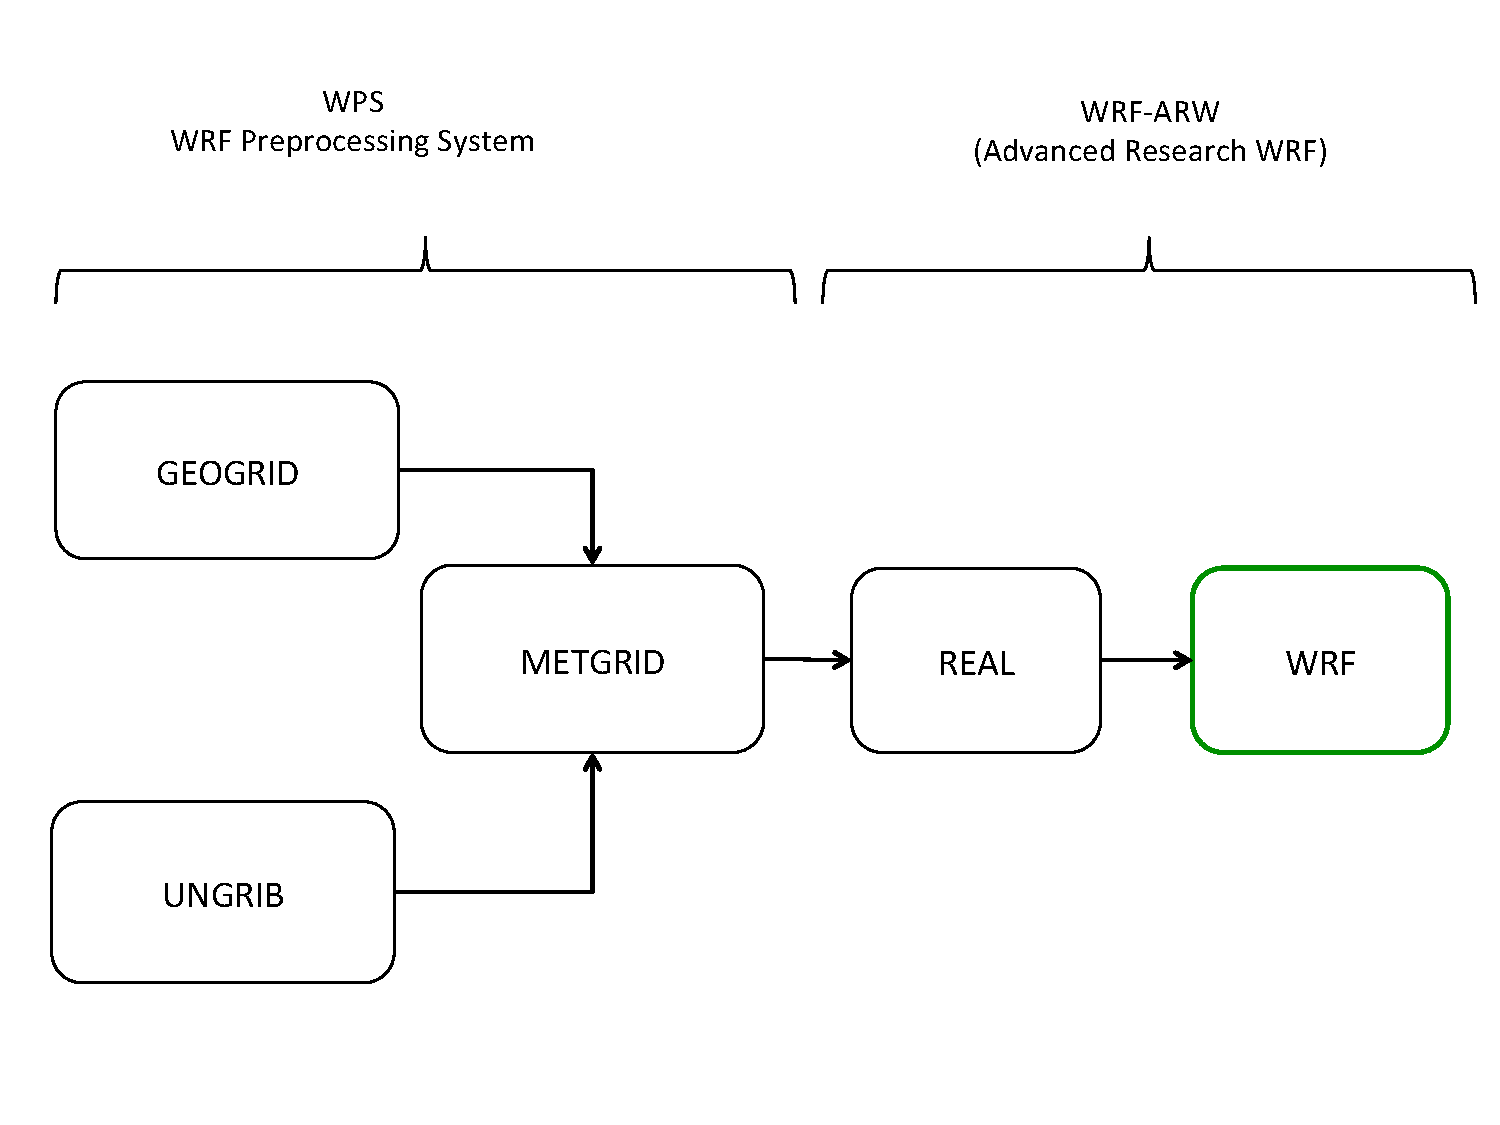
\includegraphics[scale=.35]{basic-workflow.pdf}
\end{figure}
\tiny{
\emph{Note that GEOGRID and UNGRIB are independent of each other so you may choose to run one or the other first}.
}

\end{frame}

%-------------------------------------------------------------------------------------------------------------------
\begin{frame}[fragile]\frametitle{Required files for basic workflow}

Copy the basic workflow files to \textbf{RUNDIR}:
\begin{lstlisting}
> cp -r $PROJECTDIR/tutorial/basic_workflow $RUNDIR

Where:
common.reg : shared script with settings used by other scripts.
*.reg : scripts to run pre-processors and model.
namelist* : namelist files required by executables.
data/ungrib/* : GRIB atmospheric data for initial conditions used by UNGRIB component.
\end{lstlisting}

\textbf{Note}: All workflows described in this tutorial are part of a small database of testcases used for NU-WRF regression testing.  Such tests are executed using the \textbf{reg} script located in scripts/python/regression and can be used to generate/setup the files in each testcase~(hence the \emph{reg} extension of the script files). For more information see section~\ref{sec:reg_testing}.

\end{frame}

%-------------------------------------------------------------------------------------------------------------------
\begin{frame}[fragile]
\frametitle{Required script changes}
\verbatimfont{\scriptsize}%
\begin{verbatim}
> cd $RUNDIR
\end{verbatim}
 Use your favorite editor to edit \textbf{common.reg} and change the values of NUWRFDIR and RUNDIR using the values set earlier.
\verbatimfont{\scriptsize}%
\begin{verbatim}
# *** Please make sure these settings are correct ***
# NUWRFDIR specifies the location of the NU-WRF source code
NUWRFDIR=<CHANGE THIS>
# RUNDIR specifies the location of the temporary run directory
RUNDIR=<CHANGE THIS>
\end{verbatim}
You may need to edit all the .reg files' account information and other settings. However, if you belong to group s0492 then the scripts should work without any modifications.
\verbatimfont{\scriptsize}%
\begin{verbatim}
Change account to appropriate SBU charge code:
#SBATCH --account s0942 
Change if you want to change number of nodes, hasw - to run on haswell nodes:
#SBATCH --ntasks=16 --constraint=hasw
Uncomment and set according to your needs and privileges:
##SBATCH --qos=high 
Uncomment (if desired) and substitute your e-mail here:
##SBATCH --mail-user=user@nasa.gov 
\end{verbatim}

\end{frame}

%-------------------------------------------------------------------------------------------------------------------
\begin{frame}[fragile]\frametitle{A note about namelists settings}

Things to keep in mind before we run NU-WRF components.
\mbox{}\\
\begin{itemize}
\item The length of the simulations is specified in the namelist files:
\begin{itemize}
\item In namelist.wps the length is determined by start\_date and end\_date
\item In namelist.input look for start\_ and end\_ fields. 
\item The dates in both namelists must be consistent.
\end{itemize}
\item The workflow is designed to work as-is. However, if you want to run for different dates:
\begin{itemize}
\item You must get the corresponding atmospheric data for initial conditions. 
\item You may need to modify the namelists. For example in namelist.input, make sure end\_day - start\_day = run\_days.
\end{itemize}
\item For \textbf{any} other changes please refer to the user's guide.
\end{itemize}
\end{frame}

%-------------------------------------------------------------------------------------------------------------------
\begin{frame}[fragile]\frametitle{GEOGRID}

\scriptsize{
GEOGRID interpolates static and climatological terrestrial data (land use, albedo, vegetation greenness, etc) to each WRF grid.
\begin{itemize}
\item Input: namelist.wps
\item Output: For \emph{N} domains (max\_dom in namelist.wps), \emph{N} geo\_em files will be created.
\end{itemize}\scriptsize}    
\hrulefill\par
\scriptsize{Before running GEOGRID ensure your domain is in the right location. To do so run plotgrids\_new.ncl}
\verbatimfont{\scriptsize}%
\begin{verbatim}
> module load other/ncl-6.3.0
> ncl $NUWRFDIR/WPS/util/plotgrids_new.ncl
\end{verbatim}
\scriptsize{This is where you would edit namelist.wps to modify the domain information.
Now run GEOGRID:}
\verbatimfont{\scriptsize}%
\begin{verbatim}
> cd $RUNDIR
> sbatch geogrid.reg
\end{verbatim}
When done, check for  "Successful completion"  string in the file geogrid.slurm.out.
geogrid.log.nnnn (nnnn is the cpu number) files will also be created for tracking run failures or debugging.


\end{frame}

%-------------------------------------------------------------------------------------------------------------------
\begin{frame}[fragile]\frametitle{UNGRIB}

\scriptsize{
UNGRIB unpacks GRIB1 or GRIB2 files that contain  meteorological data (soil moisture, soil temperature, sea surface temperature, sea ice, etc) and writes specific fields in a WPS intermediate format.
\begin{itemize}
\item Input: namelist.wps  and GRIB input data.
\item Output: Several FNL* files corresponding to number of intervals (interval\_seconds) in simulation length (start/end dates).
\end{itemize}}
\scriptsize{\textbf{Notes}: 
\begin{itemize}
\item The GRIB input is referenced in the run script, ungrib.reg:
      ./link\_grib.csh data/ungrib/fnl\_*\\
\item The UNGRIB output (FNL) is determined by the settings in the WPS namelist (namelist.wps).
\item makes use of Vtables that list the fields and their GRIB codes that must be unpacked from the GRIB files.
\end{itemize}
}
\hrulefill\par
\scriptsize{To run:}
\verbatimfont{\scriptsize}%
\begin{verbatim}
> cd $RUNDIR
> ./ungrib.reg
\end{verbatim}

\end{frame}

%-------------------------------------------------------------------------------------------------------------------
\begin{frame}[fragile]\frametitle{METGRID}

\footnotesize{
METGRID horizontally interpolates the output from UNGRIB to the WRF domains, and combines it with the
output from GEOGRID/UNGRIB.
\begin{itemize}
\item Input: namelist.wps, UNGRIB output, geo\_em* files.
\item Output: Several met\_em* files corresponding to number of intervals (interval\_seconds) in simulation length (start/end dates).
\end{itemize}
}    
\hrulefill\par
\footnotesize{To run:}
\begin{lstlisting}
> cd $RUNDIR
> sbatch metgrid.reg
\end{lstlisting}
When done, check for  "Successful completion" string in the file metgrid.slurm.out. metgrid.log.nnnn (nnnn is the cpu number) files also be created for tracking run failures or debugging.


\end{frame}

%-------------------------------------------------------------------------------------------------------------------
\begin{frame}[fragile]\frametitle{REAL}

\footnotesize{
REAL vertically interpolates the METGRID output to the WRF grid, and creates initial and lateral boundary condition files.
\begin{itemize}
\item Input: namelist.input, met\_em*  files, geo\_em* files.
\item Output: wrfinput* files (one for each domain), wrfbdy\_d01.
\end{itemize}
}    
\hrulefill\par
\footnotesize{To run:}
\begin{lstlisting}
> cd $RUNDIR
> sbatch real.reg
\end{lstlisting}
Check real.slurm.out for run completion.
If necessary check the real\_logs directory for real.rsl.out.nnnn and real.rsl.error.nnnn files.


\end{frame}

%-------------------------------------------------------------------------------------------------------------------
\begin{frame}[fragile]\frametitle{WRF}

\footnotesize{
This program will perform a numerical weather prediction simulation using the data from REAL.
\begin{itemize}
\item Input: namelist.input, wrfinput* files (one for each domain), wrfbdy\_d01.
\item Output: wrfout* files (one for each domain).
\end{itemize}
}    
\hrulefill\par
\footnotesize{To run:}
\begin{lstlisting}
> cd $RUNDIR
> sbatch wrf.reg
\end{lstlisting}

Check wrf.slurm.out for run completion.
If necessary check the wrf\_logs directory for wrf.rsl.out.nnnn and wrf.rsl.error.nnnn files.

\end{frame}

%-------------------------------------------------------------------------------------------------------------------
\begin{frame}[fragile]
\frametitle{Post-processing on Discover}

Using NCVIEW:

\begin{lstlisting}
WRF output files (NETCDF4) can be viewed using a special version of ncview installed on Discover:

/usr/local/other/SLES11.1/ncview/2.1.2/intel-12.1.0.233/bin/ncview <filename>
\end{lstlisting}

\end{frame}

%-------------------------------------------------------------------------------------------------------------------
\begin{frame}[fragile]
\frametitle{Post-processing on Discover}

Using RIP (NCAR graphics). Submit the \textbf{rip} job:
\begin{lstlisting}
> cd $RUNDIR
> ./rip.bash # (or use sbatch)
> idt filename.cgm # Substitute actual filename

rip.bash will run ripdp_wrfarw and rip to generate NCAR Graphics cgm files.
idt is a NCAR Graphics executable in $NCARG_ROOT/bin
Sample RIP plot specification tables are in $NUWRFDIR/scripts/rip and are looped through by rip.bash

See http://www2.mmm.ucar.edu/wrf/users/docs/ripug.htm for info on customizing plots with RIP. 
Minor changes to rip.bash may be necessary.
\end{lstlisting}

\end{frame}

%-------------------------------------------------------------------------------------------------------------------
\begin{frame}[fragile]
\frametitle{Post-processing on Discover}

Other available community software packages are ARWPOST (for GRADS), UPP (for GRIB), and MET (for atmospheric verification)\\
\mbox{}\\
For more information on community post-processing packages available with WRF, see \\
\begin{lstlisting}
http://www2.mmm.ucar.edu/wrf/users/docs/user_guide_V3.5/users_guide_chap9.htm
\end{lstlisting}
\mbox{}\\
ARW user homepage:\\  
\begin{lstlisting}
http://www2.mmm.ucar.edu/wrf/users
\end{lstlisting}
\mbox{}\\
NUWRF specific post-processors are GSDSU (simulates satellite data) and LVT (land surface verification).

\end{frame}

%-------------------------------------------------------------------------------------------------------------------
\begin{frame}[fragile]
\frametitle{Adjustments for Pleiades}

On Pleiades set  PROJECTDIR to:
\verbatimfont{\small}%
\begin{verbatim}
> export PROJECTDIR=/nobackupp8/nuwrf
\end{verbatim}
Revise all the *.reg files and edit as needed. The scripts should work with minor modifications - if any at all, but make sure you check the following anyway:
\verbatimfont{\scriptsize}%
\begin{verbatim}
Change s0942 to appropriate SBU charge code:
#PBS -W group_list=s0942 
Change if you want to change number of nodes, "has" - to run on haswell nodes:
#PBS -l select=6:ncpus=16:mpiprocs=16:model=san
Set according to your needs and privileges:
#PBS -q devel 
\end{verbatim}
\end{frame}

